\documentclass[10pt]{article}

\usepackage{geometry}
\geometry{
	a4paper,
	total={6.85in, 9.9in},
	left=0.71in,
	top=0.63in,
}
\usepackage[utf8]{inputenc}
\usepackage{hyperref}
\usepackage{graphicx}
\linespread{0.96}

\pagenumbering{gobble}

\title{The Last 5\% Problem of Rewriting Software with AI}

\makeatletter
\renewcommand{\maketitle}{
\begin{flushleft}
{\noindent\Huge\bf\@title}\break
\end{flushleft}
}
\makeatother

\begin{document}
\maketitle

Recently, people are reverse-engineering and rewriting popular applications
like Photoshop
(PhotoCraft\footnote{\url{https://github.com/storytold/photocraft}}) and
Microsoft Word (WordCraft\footnote{\url{https://github.com/storytold/wordcraft}})
as open-source applications with the help of AI. There are a lot of discussions
around this, and I wish to focus on the last 5\% problem: even if an
open-source rewrite reaches very high fidelity, there are still likely to be
differences that cannot be easily eliminated. Those differences might become a
problem when high fidelity is a requirement for the AI rewrite.

I happened to experiment with reverse-engineering and rewriting old code with
AI earlier. The first case I want to share is my rewrite of
the Excel 2000 \textbf{Dev Hunter} Easter egg game.\footnote{\url{https://github.com/xusheng6/excel2000-devhunter-standalone}}
I previously wrote about it in \emph{Paged Out!} issue 6. It
is a hidden car-shooter game in Excel 2000. I wrote a small
\texttt{loader.exe} in assembly language that loads \texttt{MSOWC.DLL} and runs
the game. While it
works, it is imperfect because you still have to carry the Excel 2000 DLL, and
I cannot distribute that DLL due to copyright restrictions. So I wanted to
reverse-engineer and rewrite the game as a standalone program.

I thought this would probably be an easy task, but it did not turn out to be
that easy. If you look at Fig.~1, the image on the left is what I got on the
first try. It is somewhat recognizable, but the image on the right, which is
the final result, is very different. I prompted the AI to use the debugger as
a reference to observe values and calculations, and then fix the rewrite.
Eventually it reached a state I was very happy with. If you play
it, it feels similar to the original.

\begin{figure}[h]
\centering
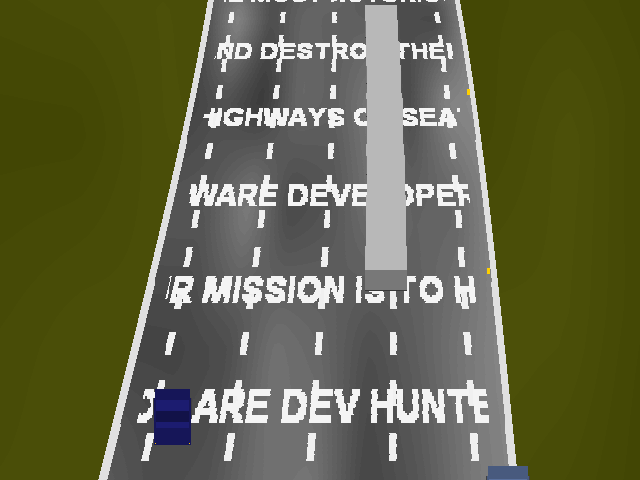
\includegraphics[width=0.35\linewidth]{before.png}\hspace{0.02\linewidth}
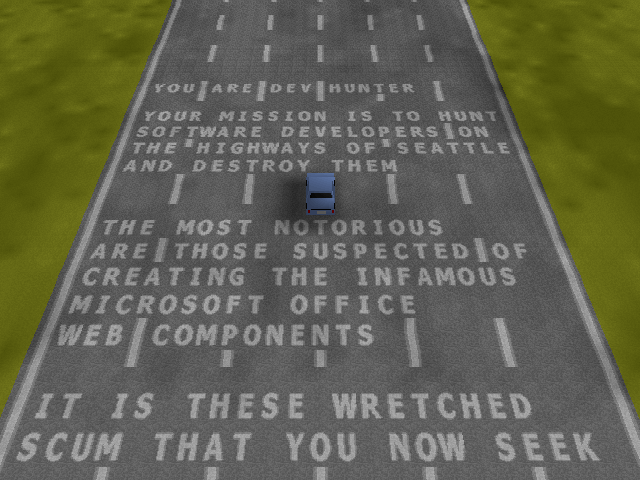
\includegraphics[width=0.35\linewidth]{after.png}
\caption{The first attempt (left) and the final result (right).}
\end{figure}

But when I looked at it more closely, I realized it was still missing two
things. There is a rainy mode that appears with a
certain probability, and the evening scene does not match exactly. None of
these differences prevent this from being a very good remake of a childhood
game I used to play. But it is still technically different from the original
game.

Someone might argue that this does not really matter because you would not
expect a game remake to be 100\% accurate. However, another project I tried
to reproduce is a little different. It is an old Chinese chess (Xiangqi)
engine.\footnote{\url{https://github.com/xusheng6/cch-cms1}} In that case, I did much the same thing: I asked the AI to analyze the
program through static reverse engineering and with the help of a debugger,
then rewrite it. It quickly got pretty close, but the remaining differences
took a long time and a lot of tokens to figure out.

I set up a loop to generate random positions, run them through the original
and rewritten engines, and compare their analyses. Whenever there was a
difference, I asked the AI to find where it came from and fix it.\footnote{My longer account of this
project: \url{https://xusheng.dev/posts/rebuilding-a-dos-xiangqi-engine/}.}

Eventually, I was satisfied that the rewritten engine matched the original on
408,708 test cases. For my purposes, that is good enough. But consider a
financial system or another critical system, where you want the rewrite to be
exactly the same as the original. How do you approach that? Do you come up
with a way to prove it? Do you use formal verification? Even if you test a
million or a billion cases and they match, you cannot be sure that the two
programs are necessarily the same. In general, there is no algorithm that can
decide whether any two arbitrary programs are equivalent.\footnote{Program-equivalence discussion:
\url{https://facultyweb.cs.wwu.edu/~wehrwes/courses/csci301_25s/lectures/L32/N32.html}}

It seems that AI can get a rewrite of an existing program started and bring it
to a point that looks right or works well in practice. Getting it to 100\%
accuracy is a very different challenge.

\end{document}
